\documentclass[12pt,a4paper,finnish
% ,twoside,openright
]{tunithesis}

% Note that you must choose either Finnish or English here and there in this
% file.
% Other options for document class
  % ,twoside,openright   % If printing on both sides (>80 pages)
  % ,twocolumn           % Can be used in lab reports, not in theses

% Ensure the correct Pdf size (not needed in all environments)
\special{papersize=210mm,297mm}


% LaTeX file for BSC/MSc theses and lab reports.
% Requires the class file (=template) tunithesis.cls and figure files,
% either tut-logo, exampleFig (as pdf or eps) and example_code.c
% Author: Lucas Machado (2018)
% Based on TTU template by Sami Paavilainen (2006), modified by Heikki Huttunen (2014)

% More information about Latex basics:
% [Tobias Oetiker, Hubert Partl, Irene Hyna, Elisabeth Schlegl, The
% Not So Short Introduction to LATEX2e, Version 5.03, April 2014, 171
% pages.  Availbale: http://tobi.oetiker.ch/lshort/lshort.pdf]

\author{Väinö-Waltteri Granat}
%\title{Zero to DLA: Building Software Support For Custom RISC-V SoC To Accelerate Deep Neural Networks} % primary title (for front page)
\title{Zero to DLA: Building Software Stack for Accelerating Deep Neural Networks on Custom RISC-V SoC} % primary title (for front page)
\thesistype{Diplomityö} % or Bachelor of Science, Laboratory Report...

% Put your thesis' main language last
% http://mirrors.ctan.org/macros/latex/required/babel/base/babel.pdf
\usepackage{lastpage}
\usepackage[finnish]{babel}
\usepackage[
backend=biber,
style=numeric-comp,
citestyle=numeric-comp,
autocite=footnote,
maxbibnames=5
]{biblatex}
\usepackage{csquotes}
\usepackage{booktabs}
\usepackage{adjustbox}
\usepackage{subcaption}
\usepackage{caption}
\usepackage{svg}
\usepackage[withpage]{acronym}
\usepackage{tikz}
\usetikzlibrary{arrows.meta, arrows}
\usetikzlibrary{matrix, positioning}
\usepackage{xcolor}
\usepackage{amsfonts}
\usepackage{listings, listings-rust}
%\usepackage{inconsolata}
\usepackage{graphicx}
\usepackage{float}
\usepackage{multirow}
\usepackage{calc}

\addbibresource{../thesis/thesis_refs.bib} %Imports bibliography file
\addbibresource{../thesis/zotero.bib} %Imports bibliography file

% Table caption on top
\floatstyle{plaintop}
\restylefloat{table}

% Fix this
\newcommand{\fixthis}[1]{\textbf{\textit{\textcolor{red}{[#1]}}}}

\definecolor{tunipurple}{RGB}{78, 0, 142}

\newcommand\todo[1]{{\color{red}!!!TODO: #1}} % Remark text in braces appears in red
\newcommand{\angs}{\textsl{\AA}}              % , e.g. slanted symbol for Ångstöm
\def\checkmark{\tikz\fill[scale=0.4](0,.35) -- (.25,0) -- (1,.7) -- (.25,.15) -- cycle;}
\def\scalecheck{\resizebox{\widthof{\checkmark}*\ratio{\widthof{x}}{\widthof{\normalsize x}}}{!}{\checkmark}}
\lstdefinestyle{customc}{
  belowcaptionskip=1\baselineskip,
  breaklines=true,
  frame=L,
  xleftmargin=\parindent,
  language=C,
  showstringspaces=false,
  basicstyle=\footnotesize\ttfamily,
  keywordstyle=\bfseries\color{green!40!black},
  commentstyle=\itshape\color{purple!40!black},
  identifierstyle=\color{blue},
  stringstyle=\color{orange},
  postbreak=\mbox{\textcolor{red}{$\hookrightarrow$}\space},
}

\lstdefinestyle{customasm}{
  belowcaptionskip=1\baselineskip,
  frame=L,
  xleftmargin=\parindent,
  language=[x86masm]Assembler,
  basicstyle=\footnotesize\ttfamily,
  commentstyle=\itshape\color{purple!40!black},
}

\lstset{escapechar=@,style=customc}

\pagenumbering{roman} % was: {Roman}
\pagestyle{headings}
\begin{document}

% Special trick so that internal macros (denoted with @ in their name)
% can be used outside the cls file (e.g. \@author)
\makeatletter

\thispagestyle{empty}
\vspace*{-.5cm}\noindent

\begin{figure}
    \vspace{-1.3cm}
    \advance\leftskip-2.5cm
    \noindent
\includegraphics{../thesis/img/tunilogo.png}
\end{figure}
 
\vspace{2.5cm}
\begin{flushright}
\noindent\textsf{\LARGE{\@author}}

\noindent\vspace{0.5cm}

\noindent\Huge{\textsf{\textbf{\textcolor{tunipurple}{\@title}}}}
\end{flushright}
\vspace{10.7cm} % adjust to 12.7 this if thesis title needs two lines

% Last some additional info to the bottom-right corner
\begin{flushright}  
    \begin{spacing}{1.0}
      \textsf{Faculty of Information Technology and Communication Sciences (ITC)\\
      \@thesistype\\
      December 2024}
    \end{spacing}
\end{flushright}

% Leave the backside of title page empty in twoside mode
\if@twoside
\clearpage
\fi

%\clearpage
\chapter*{\@aidisclaimertitle}
Artificial intelligence (AI) has been used in generating this work:


I hereby declare, that the AI-based applications used in generating this work are as follows:

\begin{center}
    \begin{tabular}{c|l}
        \toprule
        \textbf{Application} & \textbf{Version} \\
        \midrule
        OpenAi, ChatGPT-4 Turbo & April - November 2024 \\
        Microsoft Copilot & April - November 2024 \\
        \bottomrule
    \end{tabular}
\end{center}

\section*{Purpose of the use of AI}

Large language models were use as an aid for generating code for some of the Tikz diagrams presented in this thesis, with the purpose of improving the quality of the given diagrams.

Explain here \emph{in detail}, for which purpose and how AI was utilized in writing this thesis.

\section*{Parts of this work, where AI was used}

List here all chapters, sections, subsections, tables, figures and so forth,
that were generated by an AI, or that an AI had a hand in generating.

The following figures were created with a help of AI: \ref{fig:rgb-array}, \ref{fig:activation-functions}, \ref{fig:network-simple}, \ref{fig:network-residual}

\section*{Acknowledgement of risks}

I hereby acknowledge, that as the author of this work, I am fully
responsible for the contents presented in this thesis. This includes
the parts that were generated by an AI, in part or in their entirety. I
therefore also acknowledge my responsibility in the case, where use of
AI has resulted in ethical guidelines being breached.

\clearpage


% Turn off page numbering for the first pages
\pagenumbering{gobble}

% \chapter*{Abstract}

% \begin{spacing}{1.0}
% \noindent \@author: \@title\\
% \@thesistype\\
% Tampere University\\
% Master’s Degree Programme in Signal Processing and Machine Learning\\
% December 2024
% \end{spacing}
% \noindent\rule{12cm}{0.4pt}

% \vspace{0.5cm}

% % ---------------------------------------
% % Abstract and keywords
% % ---------------------------------------

% \noindent Lorem ipsum~

% \noindent\textbf{Keywords:} DLA, Deep-Learning, SoC, Virtual Prototype.

% ~

% \noindent The originality of this thesis has been checked using the Turnitin Originality Check service.


\clearpage

\section*{Lyhenteet}
\begin{acronym}
  \acro{VWW}{Visual Wake Words}
\end{acronym}


% \thispagestyle{empty}
% \listoffigures
% \listoftables
\clearpage


\setcounter{tocdepth}{3}              % How many header level are included
\tableofcontents                      % Create TOC

% The actual text begins here and page numbering changes to 1,2...
% Leave the backside of title empty in twoside mode
\if@twoside
%\newpage
\cleardoublepage
\fi


\renewcommand{\chaptername}{} % This disables the prefix 'Chapter' or
                              % 'Luku' in page headers (in 'twoside'
                              % mode)


\chapter{Kypsyysnäyte}
\label{ch:introduction}
\pagenumbering{arabic}
\setcounter{page}{1} % Start numbering from zero because command
                     % 'chapter*' does page break

Järjestelmäpiirit ovat heterogeenisen laskennan muoto, jossa yhdelle piirille sijoitetaan useita itsenäisiä komponentteja, jotka yhdessä muodostavat integroidun funktionaalisen järjestelmän.
Järjestelmäpiiri voi esimerkiksi sisältää prosessoreita, kiihdyttimiä, muistia sekä tulo- ja lähtörajapintoja.

Tässä työssä pyrittiin suunnittelemaan ja toteuttamaan ohjelmistopino konvoluutionaalisten neuroverkkojen päätelaskennan kiihdyttämiseksi Tampereen yliopiston SoC Hub -tutkimusryhmän~\cite{keelhaul} Headsail-järjestelmäpiirin sy\-vä\-op\-pi\-mis\-kiih\-dy\-tti\-me\-llä.
Tavoitteena oli kehittää ohjelmistopino, joka pystyy muuntamaan koulutetun neuroverkon Headsaililla suoritettavaan muotoon ja allokoimaan verkon konvoluutio-operaatiot suoritettaviksi syväoppimiskiihdyttimellä.

Työn toinen tavoite oli mallintaa Headsail-järjestelmäpiiri, erityisesti sen sy\-vä\-op\-pi\-mis\-kiih\-dy\-tin, virtuaalisesti Renode-järjestelmäemulaattorilla~\cite{renode}.
Tämä mahdollisti ohjelmistokehityksen aloittamisen ennen Headsail-piirien valmistumista, nopeuttaen piirien käyt\-töön\-ot\-to\-a.
Koska syväoppimiskiihdytin on SoC Hubin kehittämä, sen virtuaalista vastinetta ei löydy valmiina Renoden komponenttikirjastosta, joten se kehitettiin tämän työn aikana hyödyntäen Renoden Python-oheislaiterajapintaa.

Lopullinen ohjelmistopino koostui seuraavista komponenteista: Rust-pohjaisesta alustatukipaketista, joka tarjoaa rajapinnan Headsailin ja sen oheislaitteiden ohjelmointiin; tukipakettiin sisällytettävästä ajurista syväoppimiskiihdyttimen ohjaamiseen; TVM-koneoppimiskääntäjästä~\cite{TVM}, johon integroitiin Headsail-koo\-di\-kään\-nös\-tu\-ki; sekä Headsail-yhteensopivasta C-standaardikirjaston toteutuksesta.
Kuvassa~\ref{fig:architecture} on esitetty syväoppimiskiihdyttimen käyttöön kehitetty ohjelmistopino kokonaisuudessaan.

\begin{figure}
\centering
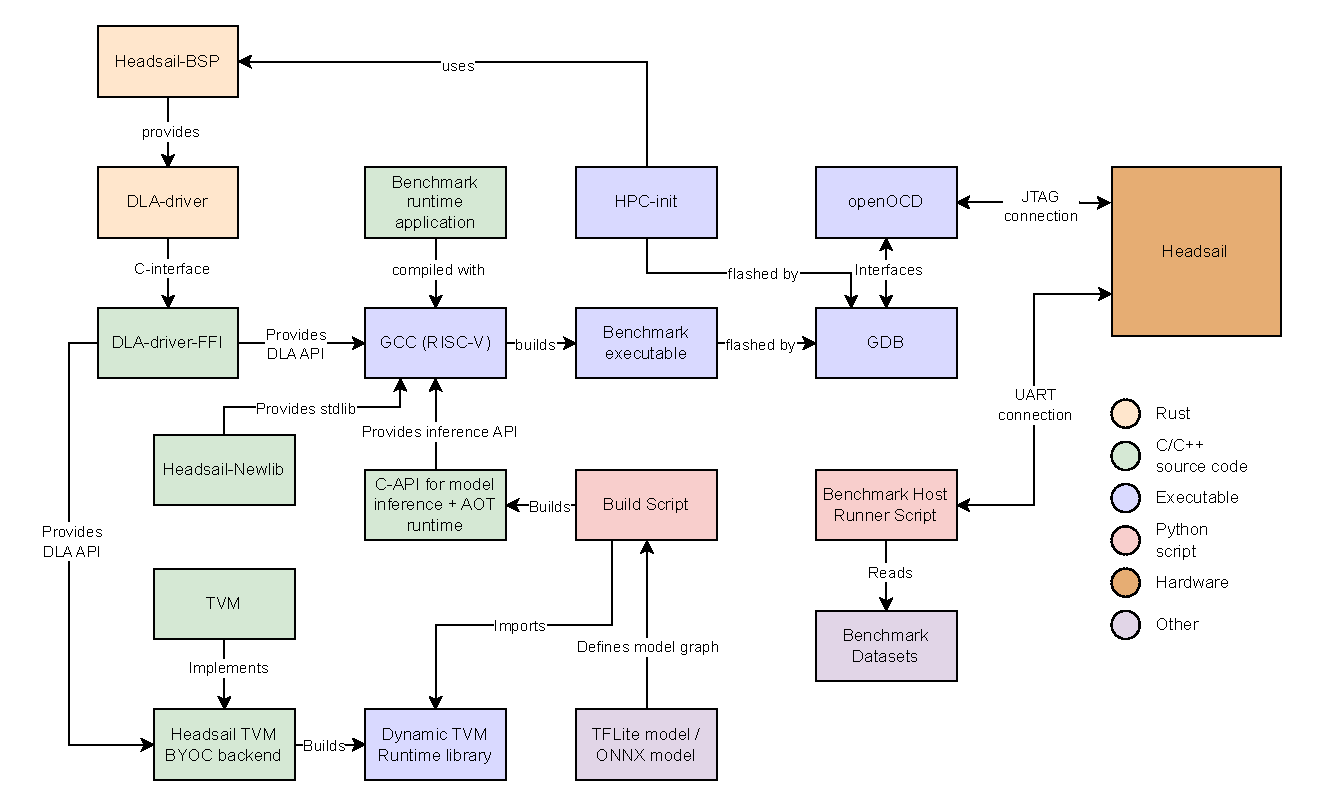
\includegraphics[width=\linewidth]{../thesis/img/dla-architecture-new.pdf}
\caption{Headsailin syvöoppimiskiihdyttimen käyttöön kehitetty ohjelmistoarkkitehtuuri.}
\label{fig:architecture}
\end{figure}

Kiihdyttimen ja sen ohjelmistopinon käyttötapaukseksi valittiin MLPerf Tiny-suorituskykytesti~\cite{banbury_mlperf_2021}, joka on päätelaskennan latenssin testaamiseen sulautetuilla alustoilla tarkoitettu avoin testikehys.
MLPerf Tiny sisältää neljä erillistä testitapausta, jotka mallintavat kiihdyttimen tosielämän käyttötapauksia tunnetuilla neuroverkkoarkkitehtuureilla.
Näistä tapauksista kolme perustuu konvoluutionaalisiin verkkoihin, siispä ne sopivat hyvin Headsailin syväoppimiskiihdyttimen testaamiseen.

Ensimmäinen käyttötapaus on avainsanojen tunnistaminen, jossa ääninäytteen logaritmisesta mel-spektrogrammista pyritään tunnistamaan yksi kahdestatoista mahdollisesta avainsanasta.
Toinen käyttötapaus on visuaalisen herätteen havaitseminen, jossa binääriluokittelevaa konvoluutionaalista verkkoa hyödyntämällä pyritään tunnistamaan, esiintyykö syötteenä annetussa kuvassa ihminen vai ei.
Viimeinen käyttötapaus on kuvan luokittelu, jossa ResNet~\cite{he_deep_2015} -neuroverkkoa hyödyntämällä pyritään luokittelemaan CIFAR-10-tietokannan kuvia oikeisiin luokkiin.

Neuroverkon kääntäminen Headsailille perustuu TVM:n kykyyn tuottaa ilman käyttöjärjestelmää suoritettavaa C-lähdekoodia, johon voidaan sisällyttää korkeantason syväoppimiskirjastoilla koulutettuja neuroverkkoja. Laajentamalla TVM:ää Headsail-yhteensopivalla koodigeneraatiomoduulilla voitiin lisätä toiminnallisuus, joka mahdollistaa C-koodin tuottamisen siten, että konvoluutiokerrokset allokoidaan suoritettavaksi syväoppimiskiihdyttimellä.

Jotta koodigeneraatio voidaan suorittaa, korkeantason neuroverkon esitys on ensin muunnettava TVM Relay -esitysmuotoon.
Relayssä neuroverkko esitetään graafina, jossa jokainen laskuoperaatio vastaa yhtä solmua ja graafin kaaret kuvaavat datan liikkumista operaatioiden välillä.
Tälle graafiesitykselle voidaan suorittaa muunnoksia, joilla neuroverkko sovitetaan kohdealustalle.
Tämän jälkeen koodigeneraatiomoduuli etsii graafista määritellyt solmukuviot, jotka on ennalta määritelty kiihdyttimellä suoritettaviksi, ja tuottaa näille C-koodia, joka käyttää alustatukipaketin konvoluutiokomentoja päätelaskennan aikana.

Valmiin ohjelmistopinon avulla suoritettiin edellä kuvatut MLPerf Tiny -suo\-ri\-tus\-ky\-ky\-tes\-tin kolme konvoluutiopohjaista käyttötapausta Headsailin virtuaalimallissa.
Teknisten ongelmien takia, testikehystä ei pystytty suorittamaan oikealla jär\-jes\-tel\-mä\-pii\-ri\-llä, eikä latenssimittausta saatu siten suoritettua. Virtuaalimallin testaaminen kuitenkin todistaa ohjelmistopinon toimivuuden ja sy\-vä\-op\-pi\-mis\-kiih\-dy\-tti\-men yhteensopivuusasteen testikehyksen referenssimallien kanssa.
Testitulosten perusteella Headsailin sy\-vä\-op\-pi\-mis\-kiih\-dy\-tin pystyi vaihtelevasti kiihdyttämään yleistapauksellisia neuroverkkoja säilyttäen referenssimallin tarkkuuden.
Vaihtelevuuden pääsyyksi havaittiin kiihdyttimen rajoitettu ulostuloleveys, joka osoittautui liian kapeaksi monille neuroverkoille.
Jotta syväoppimiskiihdyttimellä voitaisiin suorittaa neuroverkkoja paremmalla tarkkuudella, tulisi verkot kouluttaa rajoitettu ulostuloleveys erityisesti huomioonottaen.




%
% The bibliography, i.e the list of references
%
\newpage

\printbibliography[title=Lähteet]
\addcontentsline{toc}{chapter}{Lähteet}


%
% Appendices are optional. 
% This part is semi-ugly at the moment. Please give feedback if can
% improve it.

\end{document}


% LocalWords:  quantizising
